% 20120525-150822-151122
% A-7.0/W35.6

\section{A-7.0/W35.6 - 171 krpm}
\label[secinapp]{sec:awp-exp-details-A-7.0/W35.6}

This test has been performed on May 25\th{} 2012, between 15:08:22 and
15:11:22.

\begin{figure}[htbp]
  \centering
  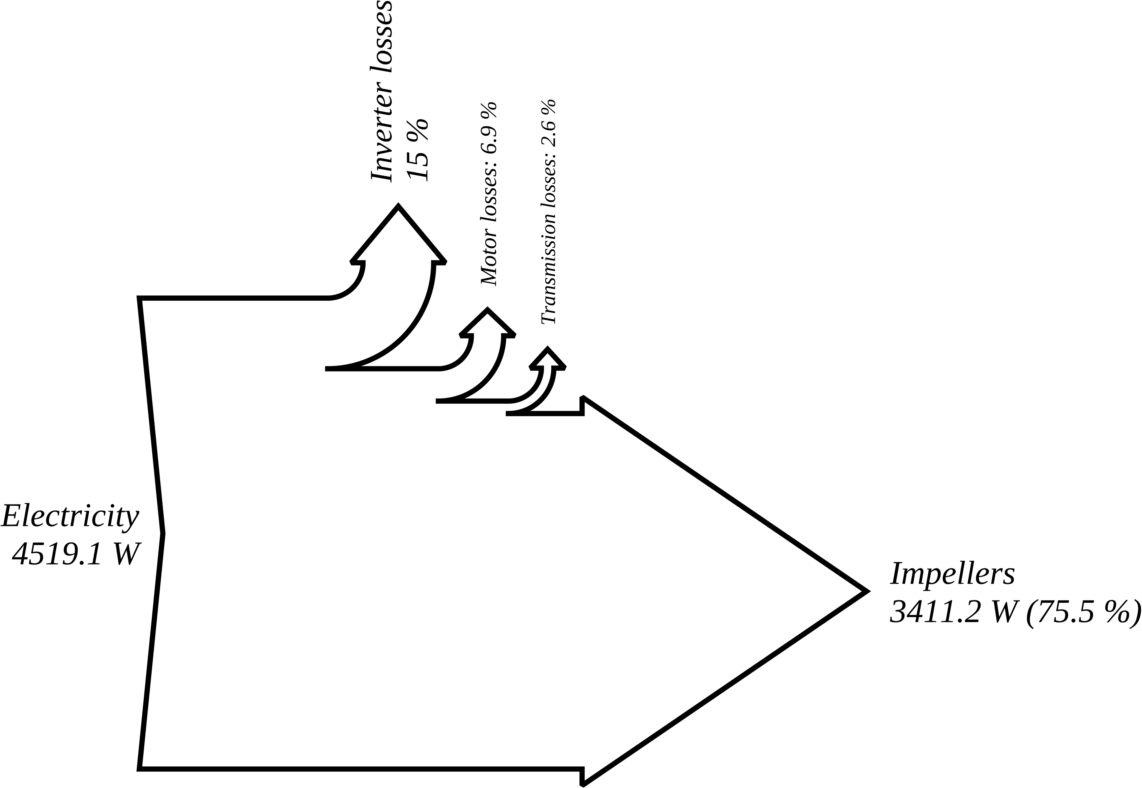
\includegraphics[width=0.7\textwidth]{awp-energy-sankey-cp-20120525-150822-151122}
  \caption{A-7.0/W35.6 -- Sankey diagram for the compressor unit energy balance}
  \label{fig:awp-A-7.0/W35.6-sankey-cp}
\end{figure}

\begin{figure}[htbp]
  \centering
  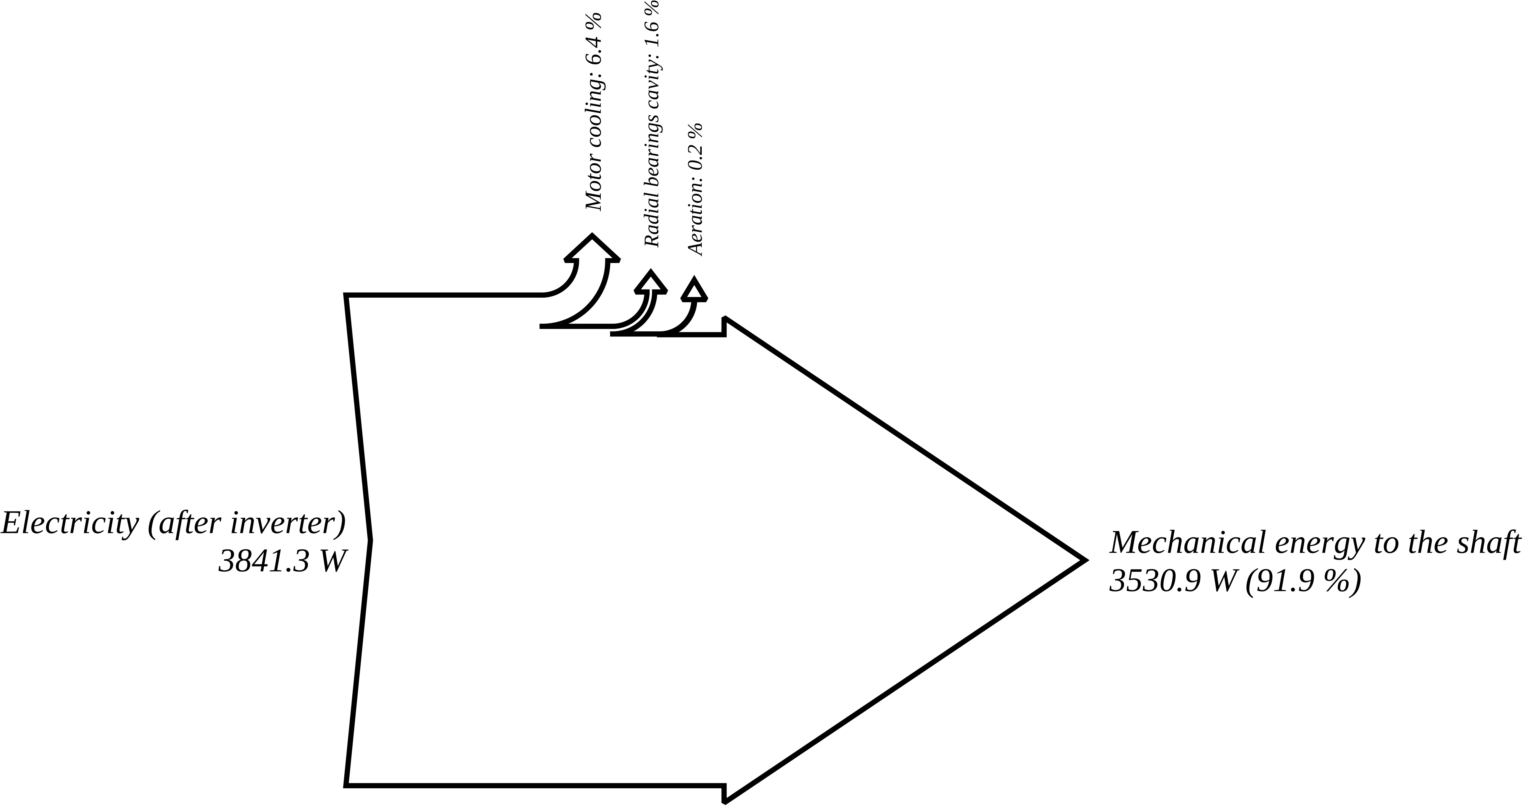
\includegraphics[width=0.7\textwidth]{awp-energy-sankey-motor-20120525-150822-151122}
  \caption{A-7.0/W35.6 -- Sankey diagram for the motor energy balance}
  \label{fig:awp-A-7.0/W35.6-sankey-motor}
\end{figure}

\begin{table}[htbp]
    \footnotesize
    \begin{center}
    \begin{tabular}{llllll}
\toprule
Name & Value / \% & Name & Value / \% & Name & Value / - \\
\midrule
$\eta_{heatpump}$ & $ \num{30.5} \pm \num{0.5} $ & $\eta_{motor}$ & $ \num{91.8} \pm \num{0.2} $ & $\epsilon_h$ & $ \num{2.36} \pm \num{2.36} $\\
$\eta_{cp1}$ & $ \num{70} \pm \num{31} $ & $\eta_{cp2}$ &$ \num{52} \pm \num{14} $ & $\pi_1$ & $ \num{2.381} \pm \num{2.381} $\\
$\eta_{cp1,\,imp}$ & $ \num{62} \pm \num{37} $ & $\eta_{cp2,\,imp}$ & $ \num{59} \pm \num{16} $ & $\pi_2$ & $ \num{2.670} \pm \num{2.670} $\\
$\eta_{cd}$ & $ \num{92} \pm \num{3} $ & $\eta_{ev}$ & $ \num{34} \pm \num{34} $ & $\pi_{1,\,theory}$ & $ \num{3.9} \pm \num{3.9} $\\
$\eta_{trans}$ & $ \num{96.61} \pm \num{0.02} $ & $\eta_{sc}$ & $ \num{2} \pm \num{2} $ & $\pi_{2,\,theory}$ & N/A\\
$\eta_{s,\,cp1}$ & $ \num{88} \pm \num{11} $ & $\eta_{s,\,cp2}$ & $ \num{82} \pm \num{18} $ & $\eta_{motor}$ & $\underline{91.92}$ \%\\
$\eta_{s,\,cp1,\,ext}$ & $ \num{98} \pm \num{3} $ & $\eta_{s,\,cp2,\,ext}$ & $ \num{68} \pm \num{32} $ & $\eta_{radial}$ & $ \num{98.75} \pm \num{0.02} $ \%\\
$\eta_{s,\,cp1,\,theory}$ & $ \num{77} \pm \num{1} $ & $\eta_{s,\,cp2,\,theory}$ & N/A & $\eta_{axial}$ & $ \num{97.83} \pm \num{0.02} $ \%\\
\bottomrule
\end{tabular}

  \end{center}
  \caption{A-7.0/W35.6 -- Performance indicators}
\end{table}

\begin{table}[htbp]
  \footnotesize
  \begin{center}
    \begin{tabular}{cccccc}
\toprule
Component & Location & P / \si{\bar} & T / \si{\degreeCelsius} & h / \si{\kilo\joule\per\kilo\gram} & s / \si{\kilo\joule\per\kilo\gram\per\kelvin}\\
\midrule
\multirow{2}{*}{1} & inlet & $ \num{1.459} \pm \num{0.001} $ & $ \num{-6} \pm \num{12} $ & $ \num{398.03} \pm \num{0.02} $ & $ \num{1.78} \pm \num{0.04} $\\
& outlet & $ \num{3.475} \pm \num{0.001} $ & $ \num{37} \pm \num{3} $ & $ \num{430.787} \pm \num{0.003} $ & $ \num{1.825} \pm \num{0.009} $\\
\midrule
\multirow{2}{*}{2} & inlet & $\pmb{ \num{3.475} \pm \num{0.001} }$ & $\pmb{ \num{11.945} \pm \num{0.006} }$ & $ \num{407.896096} \pm \num{6e-06} $ & $ \num{1.74766} \pm \num{6e-05} $\\
& outlet & $\pmb{ \num{9.278} \pm \num{0.001} }$ & $\pmb{ \num{53.358} \pm \num{0.006} }$ & $ \num{435.887724} \pm \num{6e-06} $ & $ \num{1.76869} \pm \num{4e-05} $\\
\midrule
\multirow{2}{*}{3} & inlet & $\pmb{ \num{9.076} \pm \num{0.001} }$ & $\pmb{ \num{51.868} \pm \num{0.005} }$ & $ \num{434.716360} \pm \num{5e-06} $ & $ \num{1.76661} \pm \num{3e-05} $\\
& outlet & $\pmb{ \num{8.672} \pm \num{0.001} }$ & $\pmb{ \num{33.788} \pm \num{0.005} }$ & $ \num{247.229755} \pm \num{5e-06} $ & $ \num{1.16129} \pm \num{2e-05} $\\
\midrule
\multirow{2}{*}{4} & inlet & $ \num{1.615} \pm \num{0.001} $ & $ \num{-15.4} \pm \num{0.7} $ & $ \num{248.5511} \pm \num{7e-04} $ & $ \num{1.191} \pm \num{0.002} $\\
& outlet & $\pmb{ \num{1.597} \pm \num{0.001} }$ & $\pmb{ \num{-14.971} \pm \num{0.005} }$ & $ \num{389.791392} \pm \num{5e-06} $ & $ \num{1.7397} \pm \num{1e-04} $\\
\midrule
\multirow{2}{*}{5} & inlet & $ \num{8.672} \pm \num{0.001} $ & $ \num{33.79} \pm \num{0.04} $ & $ \num{247.22976} \pm \num{4e-05} $ & $ \num{1.1613} \pm \num{2e-04} $\\
& outlet & $ \num{3.475} \pm \num{0.001} $ & $ \num{4.8} \pm \num{0.4} $ & $ \num{247.2298} \pm \num{4e-04} $ & $ \num{1.170} \pm \num{0.002} $\\
\midrule
\multirow{2}{*}{6} & inlet & $ \num{3.475} \pm \num{0.001} $ & $ \num{0} \pm \num{5} $ & $ \num{200.170} \pm \num{0.005} $ & $ \num{1.00} \pm \num{0.02} $\\
& outlet & $ \num{1.834} \pm \num{0.001} $ & $ \num{-12.3} \pm \num{0.7} $ & $ \num{200.1704} \pm \num{7e-04} $ & $ \num{1.002} \pm \num{0.003} $\\
\midrule
\multirow{2}{*}{7} & inlet & $ \num{1.834} \pm \num{0.001} $ & $ \num{-12.3} \pm \num{0.7} $ & $ \num{247.2298} \pm \num{7e-04} $ & $ \num{1.183} \pm \num{0.002} $\\
& outlet & $ \num{1.834} \pm \num{0.001} $ & $ \num{-12.3} \pm \num{0.7} $ & $ \num{257.4993} \pm \num{7e-04} $ & $ \num{1.222} \pm \num{0.002} $\\
\midrule
\multirow{2}{*}{8} & inlet & $\pmb{ \num{3.475} \pm \num{0.001} }$ & $\pmb{ \num{4.822} \pm \num{0.006} }$ & $ \num{401.390488} \pm \num{6e-06} $ & $ \num{1.7246} \pm \num{4e-04} $\\
& outlet & $ \num{3.47} \pm \num{0.05} $ & $ \num{4.8} \pm \num{0.4} $ & $ \num{206.5105} \pm \num{4e-04} $ & $ \num{1.023} \pm \num{0.002} $\\
\midrule
\multirow{2}{*}{9} & inlet & $\pmb{ \num{1.834} \pm \num{0.001} }$ & $\pmb{ \num{-12.253} \pm \num{0.005} }$ & $ \num{248.551107} \pm \num{5e-06} $ & $ \num{1.18783} \pm \num{6e-05} $\\
& outlet & $ \num{1.615} \pm \num{0.001} $ & $ \num{-15.4} \pm \num{0.7} $ & $ \num{248.5511} \pm \num{7e-04} $ & $ \num{1.191} \pm \num{0.002} $\\
\midrule
\multirow{2}{*}{10} & inlet & $ \num{9.278} \pm \num{0.001} $ & $ \num{53} \pm \num{3} $ & $ \num{435.888} \pm \num{0.002} $ & $ \num{1.769} \pm \num{0.008} $\\
& outlet & $ \num{3.475} \pm \num{0.001} $ & $ \num{142} \pm \num{94} $ & $ \num{533.3} \pm \num{0.1} $ & $ \num{2.1} \pm \num{0.2} $\\
\midrule
\multirow{2}{*}{11} & inlet & $ \num{1.459} \pm \num{0.001} $ & $ \num{89} \pm \num{38} $ & $ \num{481.99} \pm \num{0.04} $ & $ \num{2.0} \pm \num{0.1} $\\
& outlet & $ \num{1.459} \pm \num{0.001} $ & $ \num{135} \pm \num{63} $ & $ \num{527.15} \pm \num{0.07} $ & $ \num{2.2} \pm \num{0.2} $\\
\midrule
\multirow{2}{*}{12} & inlet & $ \num{3.231} \pm \num{0.001} $ & $ \num{8} \pm \num{6} $ & $ \num{405.190} \pm \num{0.006} $ & $ \num{1.74} \pm \num{0.02} $\\
& outlet & $ \num{3.231} \pm \num{0.001} $ & $ \num{58} \pm \num{35} $ & $ \num{450.69} \pm \num{0.04} $ & $ \num{1.9} \pm \num{0.1} $\\
\midrule
\multirow{2}{*}{13} & inlet & $ \num{3.238} \pm \num{0.001} $ & $ \num{2.81} \pm \num{0.07} $ & $ \num{400.23505} \pm \num{7e-05} $ & $ \num{1.72557} \pm \num{3e-05} $\\
& outlet & $ \num{3.231} \pm \num{0.001} $ & $ \num{43} \pm \num{33} $ & $ \num{436.86} \pm \num{0.04} $ & $ \num{1.8} \pm \num{0.1} $\\
\midrule
\multirow{2}{*}{15} & inlet & & $\pmb{ \num{28.766} \pm \num{0.005} }$ & \multicolumn{2}{l}{Cp = $ \num{4179.820} \pm \num{0.002} $ \si{\joule\per\kilo\gram\per\kelvin}}\\
& outlet & & $\pmb{ \num{35.608} \pm \num{0.005} }$ & \multicolumn{2}{l}{Cp = $ \num{4178.98964} \pm \num{7e-05} $ \si{\joule\per\kilo\gram\per\kelvin}}\\
\midrule
\multirow{2}{*}{16} & inlet & & $\pmb{ \num{-7.031} \pm \num{0.005} }$ & & \\
& outlet & & $\pmb{ \num{-10.899} \pm \num{0.005} }$ & & \\
\midrule
\multirow{2}{*}{18} & inlet & $ \num{1.597} \pm \num{0.001} $ & $ \num{-15.0} \pm \num{0.9} $ & $ \num{389.7914} \pm \num{9e-04} $ & $ \num{1.740} \pm \num{0.005} $\\
& outlet & $\pmb{ \num{1.459} \pm \num{0.001} }$ & $\pmb{ \num{-12.867} \pm \num{0.008} }$ & $ \num{391.968568} \pm \num{8e-06} $ & $ \num{1.7551} \pm \num{1e-04} $\\
\midrule
\multirow{2}{*}{19} & inlet & $ \num{3.475} \pm \num{0.001} $ & $ \num{4.8} \pm \num{0.2} $ & $ \num{206.5105} \pm \num{2e-04} $ & $ \num{1.023} \pm \num{0.001} $\\
& outlet & $ \num{3.475} \pm \num{0.001} $ & $ \num{0} \pm \num{5} $ & $ \num{200.170} \pm \num{0.005} $ & $ \num{1.00} \pm \num{0.02} $\\
\midrule
\multirow{2}{*}{20} & inlet & $ \num{9.278} \pm \num{0.001} $ & $ \num{53} \pm \num{3} $ & $ \num{435.888} \pm \num{0.002} $ & $ \num{1.769} \pm \num{0.008} $\\
& outlet & $ \num{9.076} \pm \num{0.001} $ & $ \num{52} \pm \num{3} $ & $ \num{434.716} \pm \num{0.002} $ & $ \num{1.767} \pm \num{0.008} $\\
\midrule
\multirow{2}{*}{21} & inlet & $ \num{3.238} \pm \num{0.001} $ & $ \num{2.81} \pm \num{0.07} $ & $ \num{400.23505} \pm \num{7e-05} $ & $ \num{1.72557} \pm \num{3e-05} $\\
& outlet & $\pmb{ \num{3.231} \pm \num{0.001} }$ & $\pmb{ \num{2.811} \pm \num{0.006} }$ & $ \num{400.254898} \pm \num{6e-06} $ & $ \num{1.72580} \pm \num{6e-05} $\\
\midrule
\multirow{2}{*}{22} & inlet & $ \num{1.459} \pm \num{0.001} $ & $ \num{-8} \pm \num{10} $ & $ \num{396.05} \pm \num{0.02} $ & $ \num{1.77} \pm \num{0.03} $\\
& outlet & $\pmb{ \num{1.459} \pm \num{0.001} }$ & $\pmb{ \num{-7.905} \pm \num{0.006} }$ & $ \num{396.054910} \pm \num{6e-06} $ & $ \num{1.7706} \pm \num{1e-04} $\\
\midrule
\multirow{2}{*}{23} & inlet & $ \num{1.459} \pm \num{0.001} $ & $ \num{135} \pm \num{63} $ & $ \num{527.15} \pm \num{0.07} $ & $ \num{2.2} \pm \num{0.2} $\\
& outlet & $ \num{1.459} \pm \num{0.001} $ & $ \num{152} \pm \num{71} $ & $ \num{545.25} \pm \num{0.08} $ & $ \num{2.2} \pm \num{0.2} $\\
\midrule
\multirow{2}{*}{24} & inlet & $ \num{1.459} \pm \num{0.001} $ & $ \num{56} \pm \num{36} $ & $ \num{450.69} \pm \num{0.04} $ & $ \num{2.0} \pm \num{0.1} $\\
& outlet & $ \num{1.459} \pm \num{0.001} $ & $ \num{89} \pm \num{38} $ & $ \num{481.99} \pm \num{0.04} $ & $ \num{2.0} \pm \num{0.1} $\\
\midrule
\multirow{2}{*}{25} & inlet & $ \num{3.475} \pm \num{0.001} $ & $ \num{37} \pm \num{25} $ & $ \num{449.78} \pm \num{0.03} $ & $ \num{1.88} \pm \num{0.07} $\\
& outlet & $\pmb{ \num{3.475} \pm \num{0.001} }$ & $\pmb{ \num{57.767} \pm \num{0.006} }$ & $ \num{449.776941} \pm \num{6e-06} $ & $ \num{1.88384} \pm \num{5e-05} $\\
\midrule
\multirow{2}{*}{26} & inlet & $ \num{9.278} \pm \num{0.001} $ & $ \num{53} \pm \num{3} $ & $ \num{435.888} \pm \num{0.002} $ & $ \num{1.769} \pm \num{0.008} $\\
& outlet & $\pmb{ \num{3.238} \pm \num{0.001} }$ & $\pmb{ \num{2.811} \pm \num{0.006} }$ & $ \num{400.235046} \pm \num{6e-06} $ & $ \num{1.725574} \pm \num{6e-06} $\\
\midrule
\multirow{2}{*}{27} & inlet & $ \num{3.475} \pm \num{0.001} $ & $ \num{37} \pm \num{3} $ & $ \num{430.787} \pm \num{0.003} $ & $ \num{1.825} \pm \num{0.008} $\\
& outlet & $ \num{3.475} \pm \num{0.001} $ & $ \num{37} \pm \num{3} $ & $ \num{430.787} \pm \num{0.003} $ & $ \num{1.825} \pm \num{0.008} $\\
\midrule
\multirow{2}{*}{28} & inlet & $ \num{3.475} \pm \num{0.001} $ & $ \num{4.8} \pm \num{0.4} $ & $ \num{401.3905} \pm \num{4e-04} $ & $ \num{1.725} \pm \num{0.001} $\\
& outlet & $ \num{3.475} \pm \num{0.001} $ & $ \num{12} \pm \num{4} $ & $ \num{407.896} \pm \num{0.004} $ & $ \num{1.75} \pm \num{0.01} $\\
\midrule
\multirow{2}{*}{29} & inlet & $ \num{1.459} \pm \num{0.001} $ & $ \num{-12} \pm \num{5} $ & $ \num{392.867} \pm \num{0.005} $ & $ \num{1.76} \pm \num{0.02} $\\
& outlet & $ \num{1.459} \pm \num{0.001} $ & $ \num{-6} \pm \num{11} $ & $ \num{397.26} \pm \num{0.02} $ & $ \num{1.78} \pm \num{0.04} $\\
\bottomrule
\end{tabular}

  \end{center}
  \caption{A-7.0/W35.6 -- Thermodynamic points of the heat pump cycle}
\end{table}


\begin{table}[htbp]
    \footnotesize
    \begin{center}
    \begin{tabular}{llllll}
\toprule
Name & Value / \si{\gram\per\second} & Name & Value / \si{\gram\per\second} & Name & Value / \si{\gram\per\second} \\
\midrule
$\dot{M}_{1 \rightarrow 25}$ & $ \num{29.4} \pm \num{0.9} $ & $\dot{M}_{2 \rightarrow 10}$ & $\underline{6.69}$ & $\dot{M}_{2 \rightarrow 20}$ & $ \num{57} \pm \num{1} $ \\
$\dot{M}_{2 \rightarrow 26}$ & $\pmb{ \num{1.20} \pm \num{1.20} }$ & $\dot{M}_{3 \rightarrow 5}$ & $ \num{33} \pm \num{2} $ & $\dot{M}_{3 \rightarrow 7}$ & $\pmb{ \num{23.8} \pm \num{0.3} }$ \\
$\dot{M}_{4 \rightarrow 18}$ & $ \num{28.2} \pm \num{0.9} $ & $\dot{M}_{5 \rightarrow 8}$ & $ \num{33} \pm \num{2} $ & $\dot{M}_{6 \rightarrow 9}$ & $ \num{4.4} \pm \num{4.4} $ \\
$\dot{M}_{7 \rightarrow 9}$ & $ \num{23.8} \pm \num{0.3} $ & $\dot{M}_{8 \rightarrow 19}$ & $ \num{4.4} \pm \num{4.4} $ & $\dot{M}_{8 \rightarrow 28}$ & $ \num{50} \pm \num{2} $ \\
$\dot{M}_{9 \rightarrow 4}$ & $ \num{28.2} \pm \num{0.9} $ & $\dot{M}_{10 \rightarrow 25}$ & $6.69$ & $\dot{M}_{11 \rightarrow 22}$ & $ \num{0.31} \pm \num{0.31} $ \\
$\dot{M}_{11 \rightarrow 23}$ & $ \num{0.89} \pm \num{0.89} $ & $\dot{M}_{12 \rightarrow 24}$ & $ \num{1.20} \pm \num{1.20} $ & $\dot{M}_{13 \rightarrow 12}$ & $ \num{0.162} \pm \num{0.162} $ \\
$\dot{M}_{17 \rightarrow 15}$ & $\pmb{ \num{376} \pm \num{4} }$ & $\dot{M}_{18 \rightarrow 22}$ & $ \num{28.2} \pm \num{0.9} $ & $\dot{M}_{19 \rightarrow 6}$ & $ \num{4.4} \pm \num{4.4} $ \\
$\dot{M}_{20 \rightarrow 3}$ & $ \num{57} \pm \num{1} $ & $\dot{M}_{21 \rightarrow 12}$ & $ \num{1.04} \pm \num{1.04} $ & $\dot{M}_{22 \rightarrow 29}$ & $ \num{28.5} \pm \num{0.9} $ \\
$\dot{M}_{23 \rightarrow 29}$ & $ \num{0.89} \pm \num{0.89} $ & $\dot{M}_{24 \rightarrow 11}$ & $ \num{1.20} \pm \num{1.20} $ & $\dot{M}_{25 \rightarrow 8}$ & $ \num{21.8} \pm \num{0.5} $ \\
$\dot{M}_{25 \rightarrow 27}$ & $ \num{14.3} \pm \num{0.4} $ & $\dot{M}_{26 \rightarrow 13}$ & $ \num{0.162} \pm \num{0.162} $ & $\dot{M}_{26 \rightarrow 21}$ & $ \num{1.04} \pm \num{1.04} $ \\
$\dot{M}_{27 \rightarrow 28}$ & $ \num{14.3} \pm \num{0.4} $ & $\dot{M}_{28 \rightarrow 2}$ & $ \num{65} \pm \num{2} $ & $\dot{M}_{29 \rightarrow 1}$ & $ \num{29.4} \pm \num{0.9} $ \\
$\dot{M}_{cp_1}$ & $ \num{29.4} \pm \num{0.9} $ & $\dot{M}_{cp_2}$ & $ \num{65} \pm \num{1} $ \\
\bottomrule
\end{tabular}

  \end{center}
  \caption{A-7.0/W35.6 -- Mass flow rates between the components}
\end{table}

\begin{table}[htbp]
    \footnotesize
    \begin{center}
    \begin{tabular}{llll}
\toprule
Name & Value / $W$ & Name & Value / $W$ \\
\midrule
$\dot{E}_{1 \rightarrow 2}$ & $ \num{2447} \pm \num{652} $ & $\dot{E}_{11 \rightarrow 1}$ & $ \num{3411.2} \pm \num{0.3} $ \\
$\dot{E}_{12 \rightarrow 11}$ & $ \num{3486.7} \pm \num{0.3} $ & $\dot{E}_{13 \rightarrow 12}$ & $ \num{3530.9} \pm \num{0.3} $ \\
$\dot{E}_{14 \rightarrow 13}$ & $ \num{3841.3} \pm \num{0.3} $ & $\dot{E}_{el \rightarrow 14}$ & $\pmb{ \num{4519.1} \pm \num{0.4} }$ \\
$\dot{Y}_{1 \rightarrow 2}$ & $ \num{17} \pm \num{17} $ & $\dot{Y}_{2 \rightarrow 10}$ & $ \num{652} \pm \num{652} $ \\
$\dot{Y}_{3 \rightarrow 15}$ & $ \num{1.0656e+04} \pm \num{137} $ & $\dot{Y}_{11 \rightarrow 1}$ & $ \num{17} \pm \num{17} $ \\
$\dot{Y}_{11 \rightarrow 23}$ & $ \num{16} \pm \num{16} $ & $\dot{Y}_{11 \rightarrow 24}$ & $ \num{38} \pm \num{38} $ \\
$\dot{Y}_{12 \rightarrow 11}$ & $ \num{49} \pm \num{49} $ & $\dot{Y}_{13 \rightarrow 7}$ & $ \num{244.72} \pm \num{0.02} $ \\
$\dot{Y}_{13 \rightarrow 12}$ & $ \num{59.715} \pm \num{59.715} $ & $\dot{Y}_{14 \rightarrow at}$ & $ \num{677.87} \pm \num{0.05} $ \\
$\dot{Y}_{16 \rightarrow 4}$ & $ \num{6791} \pm \num{152} $ & $\dot{Y}_{19 \rightarrow 18}$ & $ \num{61} \pm \num{61} $ \\
$\dot{Y}_{20 \rightarrow at}$ & $ \num{67} \pm \num{67} $ & $\dot{Y}_{21 \rightarrow at}$ & $ \num{0.02} \pm \num{0.02} $ \\
$\dot{Y}_{26 \rightarrow at}$ & $ \num{43} \pm \num{4} $ \\
\bottomrule
\end{tabular}

  \end{center}
  \caption{A-7.0/W35.6 -- Energy rates between the components}
\end{table}

\FloatBarrier
